\documentclass[aspectratio=169]{beamer}\usepackage[]{graphicx}\usepackage[]{xcolor}
% maxwidth is the original width if it is less than linewidth
% otherwise use linewidth (to make sure the graphics do not exceed the margin)
\makeatletter
\def\maxwidth{ %
  \ifdim\Gin@nat@width>\linewidth
    \linewidth
  \else
    \Gin@nat@width
  \fi
}
\makeatother

\definecolor{fgcolor}{rgb}{0.345, 0.345, 0.345}
\newcommand{\hlnum}[1]{\textcolor[rgb]{0.686,0.059,0.569}{#1}}%
\newcommand{\hlsng}[1]{\textcolor[rgb]{0.192,0.494,0.8}{#1}}%
\newcommand{\hlcom}[1]{\textcolor[rgb]{0.678,0.584,0.686}{\textit{#1}}}%
\newcommand{\hlopt}[1]{\textcolor[rgb]{0,0,0}{#1}}%
\newcommand{\hldef}[1]{\textcolor[rgb]{0.345,0.345,0.345}{#1}}%
\newcommand{\hlkwa}[1]{\textcolor[rgb]{0.161,0.373,0.58}{\textbf{#1}}}%
\newcommand{\hlkwb}[1]{\textcolor[rgb]{0.69,0.353,0.396}{#1}}%
\newcommand{\hlkwc}[1]{\textcolor[rgb]{0.333,0.667,0.333}{#1}}%
\newcommand{\hlkwd}[1]{\textcolor[rgb]{0.737,0.353,0.396}{\textbf{#1}}}%
\let\hlipl\hlkwb

\usepackage{framed}
\makeatletter
\newenvironment{kframe}{%
 \def\at@end@of@kframe{}%
 \ifinner\ifhmode%
  \def\at@end@of@kframe{\end{minipage}}%
  \begin{minipage}{\columnwidth}%
 \fi\fi%
 \def\FrameCommand##1{\hskip\@totalleftmargin \hskip-\fboxsep
 \colorbox{shadecolor}{##1}\hskip-\fboxsep
     % There is no \\@totalrightmargin, so:
     \hskip-\linewidth \hskip-\@totalleftmargin \hskip\columnwidth}%
 \MakeFramed {\advance\hsize-\width
   \@totalleftmargin\z@ \linewidth\hsize
   \@setminipage}}%
 {\par\unskip\endMakeFramed%
 \at@end@of@kframe}
\makeatother

\definecolor{shadecolor}{rgb}{.97, .97, .97}
\definecolor{messagecolor}{rgb}{0, 0, 0}
\definecolor{warningcolor}{rgb}{1, 0, 1}
\definecolor{errorcolor}{rgb}{1, 0, 0}
\newenvironment{knitrout}{}{} % an empty environment to be redefined in TeX

\usepackage{alltt}



\usetheme{default}
% Slide setup, colour independent

\usepackage{amsmath,amssymb,amsthm}
\usepackage[utf8]{inputenc}
\usepackage{colortbl}
\usepackage{bm}
\usepackage{xcolor}
\usepackage{dsfont}
\usepackage{setspace}
% To use \ding{234} and the like
\usepackage{pifont}
% To cross reference between slide files
\usepackage{zref-xr,zref-user}
% Use something like
% \zexternaldocument{fileI}
% in the tex files. And cite using \zref instead of \ref
\usepackage{booktabs}
\usepackage{marvosym}
\usepackage{cancel}
%\usepackage{transparent}
% Make doi clickable in the bibliography?
\usepackage{doi}

\usepackage[T1]{fontenc}

\usepackage{longtable}

% For heavier titles
\usepackage{helvet} % Enables Helvetica font family


% Fields and the like
\def\IC{\mathbb{C}}
\def\IE{\mathbb{E}}
\def\IF{\mathbb{F}}
\def\II{\mathbb{I}}
\def\IJ{\mathbb{J}}
\def\IK{\mathbb{K}}
\def\IM{\mathbb{M}}
\def\IN{\mathbb{N}}
\def\IP{\mathbb{P}}
\def\IR{\mathbb{R}}
\newcommand{\IRplus}{\mathbb{R}_{\ge 0}}
\def\IZ{\mathbb{Z}}
\def\11{\mathds{1}}


% Bold lowercase
\def\ba{\bm{a}}
\def\bb{\bm{b}}
\def\bc{\bm{c}}
\def\bd{\bm{d}}
\def\be{\bm{e}}
\def\bf{\bm{f}}
\def\bg{\bm{g}}
\def\bh{\bm{h}}
\def\bi{\bm{i}}
\def\bj{\bm{j}}
\def\bk{\bm{k}}
\def\bn{\bm{n}}
\def\bp{\bm{p}}
\def\br{\bm{r}}
\def\bs{\bm{s}}
\def\bu{\bm{u}}
\def\bv{\bm{v}}
\def\bw{\bm{w}}
\def\bx{\bm{x}}
\def\by{\bm{y}}
\def\bz{\bm{z}}
\newcommand{\vect}[1]{\bm{#1}}

% Bold capitals
\def\bB{\bm{B}}
\def\bD{\bm{D}}
\def\bE{\bm{E}}
\def\bF{\bm{F}}
\def\bG{\bm{G}}
\def\bI{\bm{I}}
\def\bL{\bm{L}}
\def\bN{\bm{N}}
\def\bP{\bm{P}}
\def\bR{\bm{R}}
\def\bS{\bm{S}}
\def\bT{\bm{T}}
\def\bX{\bm{X}}

% Bold numbers
\def\b0{\bm{0}}

% Bold greek
\bmdefine{\bmu}{\bm{\mu}}
\def\bphi{\bm{\phi}}
\def\bvarphi{\bm{\varphi}}
\def\bPi{\bm{\Pi}}
\def\bGamma{\bm{\Gamma}}

% Bold red sentence
\def\boldred#1{{\color{red}\textbf{#1}}}
\def\defword#1{{\color{orange}\textbf{#1}}}

% Caligraphic letters
\def\A{\mathcal{A}}
\def\B{\mathcal{B}}
\def\C{\mathcal{C}}
\def\D{\mathcal{D}}
\def\E{\mathcal{E}}
\def\F{\mathcal{F}}
\def\G{\mathcal{G}}
\def\H{\mathcal{H}}
\def\I{\mathcal{I}}
\def\L{\mathcal{L}}
\def\M{\mathcal{M}}
\def\N{\mathcal{N}}
\def\P{\mathcal{P}}
\def\R{\mathcal{R}}
\def\S{\mathcal{S}}
\def\T{\mathcal{T}}
\def\U{\mathcal{U}}
\def\V{\mathcal{V}}

% Adding space for prime (') where needed
\def\pprime{\,'}
% Adding space for star (\star) where needed
\def\pstar{{\,\star}}

% tt font for code
\def\code#1{{\tt #1}}

% i.e., e.g.
\def\eg{\emph{e.g.}}
\def\ie{\emph{i.e.}}


% Operators and special symbols
\def\nbOne{{\mathchoice {\rm 1\mskip-4mu l} {\rm 1\mskip-4mu l}
{\rm 1\mskip-4.5mu l} {\rm 1\mskip-5mu l}}}
\def\cov{\ensuremath{\mathsf{cov}}}
\def\Var{\ensuremath{\mathsf{Var}\ }}
\def\Im{\textrm{Im}\;}
\def\Re{\textrm{Re}\;}
\def\det{\ensuremath{\mathsf{det}}}
\def\diag{\ensuremath{\mathsf{diag}}}
\def\nullspace{\ensuremath{\mathsf{null}}}
\def\nullity{\ensuremath{\mathsf{nullity}}}
\def\rank{\ensuremath{\mathsf{rank}}}
\def\range{\ensuremath{\mathsf{range}}}
\def\sgn{\ensuremath{\mathsf{sgn}}}
\def\Span{\ensuremath{\mathsf{span}}}
\def\tr{\ensuremath{\mathsf{tr}}}
\def\imply{$\Rightarrow$}
\def\restrictTo#1#2{\left.#1\right|_{#2}}
\newcommand{\parallelsum}{\mathbin{\!/\mkern-5mu/\!}}
\def\dsum{\mathop{\displaystyle \sum }}%
\def\dind#1#2{_{\substack{#1\\ #2}}}

\newcommand{\Qmatrix}[1]{%
  \begin{pmatrix}#1\end{pmatrix}%
}

\DeclareMathOperator{\GL}{GL}
\DeclareMathOperator{\Rel}{Re}
\def\Nt#1{\left|\!\left|\!\left|#1\right|\!\right|\!\right|}
\newcommand{\tripbar}{|\! |\! |}



% The beamer bullet (in base colour)
\def\bbullet{\leavevmode\usebeamertemplate{itemize item}\ }

% Theorems and the like
\newtheorem{proposition}[theorem]{Proposition}
\newtheorem{property}[theorem]{Property}
\newtheorem{importantproperty}[theorem]{Property}
\newtheorem{importanttheorem}[theorem]{Theorem}
%\newtheorem{lemma}[theorem]{Lemma}
%\newtheorem{corollary}[theorem]{Corollary}
\newtheorem{remark}[theorem]{Remark}
\setbeamertemplate{theorems}[numbered]
%\setbeamertemplate{theorems}[ams style]

%
%\usecolortheme{orchid}
%\usecolortheme{orchid}

\def\red{\color[rgb]{1,0,0}}
\def\blue{\color[rgb]{0,0,1}}
\def\green{\color[rgb]{0,1,0}}

% Fix skipping lines after items in the bibliography
\setbeamertemplate{bibliography entry title}{}
\setbeamertemplate{bibliography entry location}{}
\setbeamertemplate{bibliography entry note}{}

% Get rid of navigation stuff
\setbeamertemplate{navigation symbols}{}

% Set footline/header line
\setbeamertemplate{footline}
{%
\quad p. \insertpagenumber \quad--\quad \insertsection\vskip2pt
}
% \setbeamertemplate{headline}
% {%
% \quad\insertsection\hfill p. \insertpagenumber\quad\mbox{}\vskip2pt
% }


\makeatletter
\newlength\beamerleftmargin
\setlength\beamerleftmargin{\Gm@lmargin}
\makeatother

% Colours for special pages
\def\extraContent{yellow!20}


%%%%%%%%%%%%%%%%%
\usepackage{tikz}
\usetikzlibrary{shapes,arrows}
\usetikzlibrary{positioning}
\usetikzlibrary{shapes.symbols,shapes.callouts,patterns}
\usetikzlibrary{calc,fit}
\usetikzlibrary{backgrounds}
\usetikzlibrary{decorations.pathmorphing,fit,petri}
\usetikzlibrary{automata}
\usetikzlibrary{fadings}
\usetikzlibrary{patterns,hobby}
\usetikzlibrary{backgrounds,fit,petri}
\usetikzlibrary{tikzmark}

\usepackage{pgfplots}
\pgfplotsset{compat=1.6}
\pgfplotsset{ticks=none}

\usetikzlibrary{decorations.markings}
\usetikzlibrary{arrows.meta}
\tikzset{>=stealth}

% For tikz
\tikzstyle{cloud} = [draw, ellipse,fill=red!20, node distance=0.87cm,
minimum height=2em]
\tikzstyle{line} = [draw, -latex']


%%% For max frame images
\newenvironment{changemargin}[2]{%
\begin{list}{}{%
\setlength{\topsep}{0pt}%
\setlength{\leftmargin}{#1}%
\setlength{\rightmargin}{#2}%
\setlength{\listparindent}{\parindent}%
\setlength{\itemindent}{\parindent}%
\setlength{\parsep}{\parskip}%
}%
\item[]}{\end{list}}


% Make one image take up the entire slide content area in beamer,.:
% centered/centred full-screen image, with title:
% This uses the whole screen except for the 1cm border around it
% all. 128x96mm
\newcommand{\titledFrameImage}[2]{
\begin{frame}{#1}
%\begin{changemargin}{-1cm}{-1cm}
\begin{center}
\includegraphics[width=108mm,height=\textheight,keepaspectratio]{#2}
\end{center}
%\end{changemargin}
\end{frame}
}

% Make one image take up the entire slide content area in beamer.:
% centered/centred full-screen image, no title:
% This uses the whole screen except for the 1cm border around it
% all. 128x96mm
\newcommand{\plainFrameImage}[1]{
\begin{frame}[plain]
%\begin{changemargin}{-1cm}{-1cm}
\begin{center}
\includegraphics[width=108mm,height=76mm,keepaspectratio]{#1}
\end{center}
%\end{changemargin}
\end{frame}
}

% Make one image take up the entire slide area, including borders, in beamer.:
% centered/centred full-screen image, no title:
% This uses the entire whole screen
\newcommand{\maxFrameImage}[1]{
\begin{frame}[plain]
\begin{changemargin}{-1cm}{-1cm}
\begin{center}
\includegraphics[width=\paperwidth,height=\paperheight,keepaspectratio]
{#1}
\end{center}
\end{changemargin}
\end{frame}
}

% This uses the entire whole screen (to include in frame)
\newcommand{\maxFrameImageNoFrame}[1]{
\begin{changemargin}{-1cm}{-1cm}
\begin{center}
\includegraphics[width=\paperwidth,height=0.99\paperheight,keepaspectratio]
{#1}
\end{center}
\end{changemargin}
}

% Make one image take up the entire slide area, including borders, in beamer.:
% centered/centred full-screen image, no title:
% This uses the entire whole screen
\newcommand{\maxFrameImageColor}[2]{
\begin{frame}[plain]
\setbeamercolor{normal text}{bg=#2!20}
\begin{changemargin}{-1cm}{-1cm}
\begin{center}
\includegraphics[width=\paperwidth,height=\paperheight,keepaspectratio]
{#1}
\end{center}
\end{changemargin}
\end{frame}
}


\usepackage{tikz}
\usetikzlibrary{patterns,hobby}
\usepackage{pgfplots}
\pgfplotsset{compat=1.6}
\pgfplotsset{ticks=none}

\usetikzlibrary{backgrounds}
\usetikzlibrary{decorations.markings}
\usetikzlibrary{arrows.meta}
\tikzset{>=stealth}

\tikzset{
  clockwise arrows/.style={
    postaction={
      decorate,
      decoration={
        markings,
        mark=between positions 0.1 and 0.9 step 40pt with {\arrow{>}},
   }}}}


% Beginning of a section
\newcommand{\newSectionSlide}[1]{
\begin{frame}[noframenumbering,plain]
  \begin{tikzpicture}[remember picture,overlay]
    \node[above right,inner sep=0pt,opacity=0.2] at (current page.south west)
    {
        \includegraphics[height=\paperheight,width=\paperwidth]{#1}
    };
  \end{tikzpicture}
  \setbeamercolor{section in toc}{fg=section_page_list_colour}
  \setbeamerfont{section in toc}{size=\Large,series=\bfseries}
  \setbeamertemplate{section in toc shaded}[default][60]
  \tableofcontents[
    currentsection,
    sectionstyle=show/shaded,
    subsectionstyle=show/hide/hide,
    subsubsectionstyle=hide/hide/hide]
\end{frame}
\addtocounter{page}{-1}
}

% Beginning of a section in which we also show subsections
\newcommand{\newSectionWithSubsSlide}[1]{
	\begin{frame}[noframenumbering,plain]
		\begin{tikzpicture}[remember picture,overlay]
			\node[above right,inner sep=0pt,opacity=0.2] at (current page.south west)
			{
				\includegraphics[height=\paperheight,width=\paperwidth]{#1}
			};
		\end{tikzpicture}
		\setbeamercolor{section in toc}{fg=section_page_list_colour}
		\setbeamerfont{section in toc}{size=\Large,series=\bfseries}
		\setbeamertemplate{section in toc shaded}[default][60]
		\tableofcontents[
		currentsection,
		sectionstyle=show/hide,
		subsectionstyle=show/show/hide,
		subsubsectionstyle=hide/hide/hide]
	\end{frame}
	\addtocounter{page}{-1}
}

% Beginning of a subsection
\newcommand{\newSubSectionSlide}[1]{
\begin{frame}[noframenumbering,plain]
  \begin{tikzpicture}[remember picture,overlay]
    \node[above right,inner sep=0pt,opacity=0.2] at (current page.south west)
    {
        \includegraphics[height=\paperheight,width=\paperwidth]{#1}
    };
  \end{tikzpicture}
  \setbeamercolor{section in toc}{fg=subsection_page_list_colour}
  \setbeamerfont{section in toc}{size=\Large,series=\bfseries}
  \setbeamertemplate{section in toc shaded}[default][60]
  \setbeamerfont{subsection in toc}{series=\bfseries}
  \setbeamertemplate{subsection in toc shaded}[default][50]
  \tableofcontents[
    currentsection,
    sectionstyle=show/hide,
    subsectionstyle=show/shaded/hide,
    subsubsectionstyle=hide/hide/hide]
\end{frame}
\addtocounter{page}{-1}
}


% Beginning of a subsubsection
\newcommand{\newSubSubSectionSlide}[1]{
\begin{frame}[noframenumbering,plain]
  \begin{tikzpicture}[remember picture,overlay]
    \node[above right,inner sep=0pt,opacity=0.2] at (current page.south west)
    {
        \includegraphics[height=\paperheight,width=\paperwidth]{#1}
    };
  \end{tikzpicture}
  \setbeamercolor{section in toc}{fg=subsub_header_section}
  \setbeamerfont{section in toc}{size=\Large,series=\bfseries}
  \setbeamertemplate{section in toc shaded}[default][60]
  \setbeamerfont{subsection in toc}{series=\bfseries}
  \setbeamertemplate{subsection in toc shaded}[default][50]
  \setbeamertemplate{subsubsection in toc shaded}[default][50]
  \tableofcontents[
    currentsection,
    sectionstyle=show/hide,
    subsectionstyle=show/hide/hide,
    subsubsectionstyle=show/shaded/hide]
\end{frame}
\addtocounter{page}{-1}
}


   %%%%%%%%%%%
% To have links to parts in the outline
\makeatletter
\AtBeginPart{%
  \addtocontents{toc}{\protect\beamer@partintoc{\the\c@part}{\beamer@partnameshort}{\the\c@page}}%
}
%% number, shortname, page.
\providecommand\beamer@partintoc[3]{%
  \ifnum\c@tocdepth=-1\relax
    % requesting onlyparts.
    \makebox[6em]{Part #1:} \textcolor{green!30!blue}{\hyperlink{#2}{#2}}
    \par
  \fi
}
\define@key{beamertoc}{onlyparts}[]{%
  \c@tocdepth=-1\relax
}
\makeatother%

\newcommand{\nameofthepart}{}
\newcommand{\nupart}[1]%
    {   \part{#1}%
        \renewcommand{\nameofthepart}{#1}%
        {
          \setbeamercolor{background canvas}{bg=orange!50}
          \begin{frame}{#1}%\partpage 
          \hypertarget{\nameofthepart}{}\tableofcontents%
          \end{frame}
        }
    }

% This command creates a title page using TikZ only
\newcommand{\tikztitlepage}[1]{%
\begin{frame}[plain,noframenumbering]
  \begin{tikzpicture}[remember picture,overlay]
    % Background image
    \node[above right,inner sep=0pt,opacity=0.1] 
      at (current page.south west) 
      {\includegraphics[width=\paperwidth,height=\paperheight]{#1}};

    % University logo
    \node[anchor=north east, inner sep=5pt, opacity=0.9] 
      at (current page.north east)
      {
\includegraphics[width=0.2\textwidth]{FIGS-slides-admin/UM-logo-horizontal-CMYK.png}};
    
    % Title
    \node[anchor=center, align=center, 
          font=\fontsize{13}{15}\bfseries\color{UMbrown}, 
          text width=0.9\textwidth] 
          at ([yshift=2cm]current page.center)
          {\inserttitle};

      % Authors
      \node[anchor=center, align=center,
        font=\fontsize{10}{12}\bfseries\color{UMbrown},
        text width=0.7\textwidth]
        at ([yshift=0.8cm]current page.center)
        {\insertauthor};

      % Affiliation
      \node[anchor=north, align=center,
        font=\fontsize{9}{11}\color{UMbrown},
        text width=0.7\textwidth]
        at ([yshift=-0.2cm]current page.center)
        {\insertaffiliation};      
    % Date
    \node[anchor=north, align=center, 
          font=\fontsize{12}{16}\bfseries\color{UMbrown},
          text width=0.7\textwidth] 
          at ([yshift=0.2cm]current page.center)
          {\insertdate};

    % Land acknowledgement
    \node[anchor=south, align=justify, 
          font=\footnotesize, text=black, 
          text width=1.1\textwidth] 
          at ([yshift=0.5cm]current page.south)
          {The University of Manitoba campuses are located on original lands of Anishinaabeg, Ininew, Anisininew, Dakota and Dene peoples, and on the National Homeland of the Red River Métis.\\
          We respect the Treaties that were made on these territories, we acknowledge the harms and mistakes of the past, and we dedicate ourselves to move forward in partnership with Indigenous communities in a spirit of Reconciliation and collaboration.};
  \end{tikzpicture}
  \addtocounter{page}{-1}
\end{frame}
}
% The title page with figure
% \newcommand{\titlepagewithfigure}[1]{%
%   \begin{frame}[noframenumbering,plain]
%     \begin{tikzpicture}[remember picture,overlay]
%       \node[above right,inner sep=0pt,opacity=0.1] at (current page.south west)
%       {
%           \includegraphics[height=\paperheight,width=\paperwidth]{#1}
%       };
%       \node[anchor=north east,
%       inner sep=5pt,
%       opacity=0.9] at (current page.north east)
%       {
%           
\includegraphics[width=0.2\textwidth]{FIGS-slides-admin/UM-logo-horizontal-CMYK.png}
%       };
%       \node[anchor=south, 
%       align=justify, 
%       text=black, 
%       text width=1.1\textwidth,
%       font=\footnotesize]  (land_acknowledgement)
%       at (current page.south) 
%       {The University of Manitoba campuses are located on original lands of Anishinaabeg, Ininew, Anisininew, Dakota and Dene peoples, and on the National Homeland of the Red River Métis.
%       We respect the Treaties that were made on these territories, we acknowledge the harms and mistakes of the past, and we dedicate ourselves to move forward in partnership with Indigenous communities in a spirit of Reconciliation and collaboration.};  
%       % \node[align=center, anchor=south,
%       % above=0.5cm of land_acknowledgement,
%       % text=black,
%       % font=\bfseries] {\insertdate};
%   \end{tikzpicture}
%   \setbeamercolor{title}{fg=title_page_title_colour}
%   \setbeamerfont{title}{size=\Large,series=\bfseries}
%   \setbeamercolor{author}{fg=title_page_author_colour}
%   \setbeamerfont{author}{size=\large,series=\bfseries}
%   \setbeamercolor{institute}{fg=title_page_institute_colour}
%   \setbeamerfont{institute}{size=\large,series=\bfseries}
%   \setbeamercolor{date}{fg=title_page_date_colour}
%   \setbeamerfont{date}{series=\bfseries}
% 	\titlepage
% \end{frame}
% \addtocounter{page}{-1}
% }

\newcommand{\titlepagewithfigure}[1]{%
  \begin{frame}[noframenumbering,plain]
    \begin{tikzpicture}[remember picture,overlay]
      \node[above right,inner sep=0pt,opacity=0.1] at (current page.south west)
      {
          \includegraphics[height=\paperheight,width=\paperwidth]{#1}
      };
      \node[anchor=north east,
      inner sep=5pt,
      opacity=0.9] at (current page.north east)
      {
          
\includegraphics[width=0.2\textwidth]{FIGS-slides-admin/UM-logo-horizontal-CMYK.png}
      };
      \node[anchor=south, 
      align=justify, 
      text=black, 
      text width=1.1\textwidth,
      font=\footnotesize]  (land_acknowledgement)
      at (current page.south) 
      {The University of Manitoba campuses are located on original lands of Anishinaabeg, Ininew, Anisininew, Dakota and Dene peoples, and on the National Homeland of the Red River Métis.
      We respect the Treaties that were made on these territories, we acknowledge the harms and mistakes of the past, and we dedicate ourselves to move forward in partnership with Indigenous communities in a spirit of Reconciliation and collaboration.};  
      % \node[align=center, anchor=south,
      % above=0.5cm of land_acknowledgement,
      % text=black,
      % font=\bfseries] {\insertdate};
  \end{tikzpicture}
  \setbeamercolor{title}{fg=title_page_title_colour}
  \setbeamerfont{title}{size=\Large,series=\bfseries,family=\usefont{T1}{phv}{b}{n}}
  \setbeamercolor{author}{fg=title_page_author_colour}
  \setbeamerfont{author}{size=\large,series=\bfseries,family=\usefont{T1}{phv}{b}{n}}
  \setbeamercolor{institute}{fg=title_page_institute_colour}
  \setbeamerfont{institute}{size=\large,series=\bfseries,family=\usefont{T1}{phv}{b}{n}}
  \setbeamercolor{date}{fg=title_page_date_colour}
  \setbeamerfont{date}{series=\bfseries,family=\usefont{T1}{phv}{b}{n}}
	\titlepage
\end{frame}
\addtocounter{page}{-1}
}
% The outline page, with figure
% \newcommand{\outlinepage}[1]{%
% \begin{frame}[noframenumbering,plain]
%   \begin{tikzpicture}[remember picture,overlay]
%     \node[above right,inner sep=0pt,opacity=0.2] at (current page.south west)
%     {
%         \includegraphics[height=\paperheight,width=\paperwidth]{#1}
%     };
%   \end{tikzpicture}
%   \setbeamercolor{section in toc}{fg=outline_page_list_colour}
%   \setbeamerfont{section in toc}{size=\Large,series=\bfseries,family=\sffamily}
%   \frametitle{\textcolor{outline_page_title_colour}{\LARGE\bfseries Outline}}
%   \tableofcontents[hideallsubsections]
% \end{frame}
% \addtocounter{page}{-1}
% }
% The outline page, with figure
\newcommand{\outlinepage}[1]{%
\begin{frame}[noframenumbering,plain]
  \begin{tikzpicture}[remember picture,overlay]
    \node[above right,inner sep=0pt,opacity=0.2] at (current page.south west)
    {
        \includegraphics[height=\paperheight,width=\paperwidth]{#1}
    };
  \end{tikzpicture}
  \setbeamercolor{section in toc}{fg=outline_page_list_colour}
  % Use Helvetica Bold only for the outline slide TOC
  \setbeamerfont{section in toc}{size=\Large,family=\usefont{T1}{phv}{b}{n}}
  % Use Helvetica Bold for the outline title
  \frametitle{\textcolor{outline_page_title_colour}{\usefont{T1}{phv}{b}{n}\LARGE Outline}}
  \tableofcontents[hideallsubsections]
\end{frame}
\addtocounter{page}{-1}
}


%\let\oldsection\section
%\renewcommand{\section}[2]{\oldsection[#1]\newSectionSlide[#2]}





\usecolortheme{orchid}
%% Listings
\usepackage{listings}
\definecolor{mygreen}{rgb}{0,0.6,0}
\definecolor{mygray}{rgb}{0.5,0.5,0.5}
\definecolor{mymauve}{rgb}{0.58,0,0.82}
\definecolor{mygold}{rgb}{1,0.843,0}
\definecolor{myblue}{rgb}{0.537,0.812,0.941}

\definecolor{mygold2}{RGB}{120,105,22}
\definecolor{mygrey2}{RGB}{50,50,50}

\definecolor{lgreen}{rgb}{0.6,0.9,.6}
\definecolor{lred}{rgb}{1,0.5,.5}

\lstloadlanguages{R}
\lstset{ %
  language=R,
  backgroundcolor=\color{black!05},   % choose the background color
  basicstyle=\footnotesize\ttfamily,        % size of fonts used for the code
  breaklines=true,                 % automatic line breaking only at whitespace
  captionpos=b,                    % sets the caption-position to bottom
  commentstyle=\color{mygreen},    % comment style
  escapeinside={\%*}{*)},          % if you want to add LaTeX within your code
  keywordstyle=\color{red},       % keyword style
  stringstyle=\color{mygold},     % string literal style
  keepspaces=true,
  columns=fullflexible,
  tabsize=4,
}
% Could also do (in lstset)
% basicstyle==\fontfamily{pcr}\footnotesize
\lstdefinelanguage{Renhanced}%
  {keywords={abbreviate,abline,abs,acos,acosh,action,add1,add,%
      aggregate,alias,Alias,alist,all,anova,any,aov,aperm,append,apply,%
      approx,approxfun,apropos,Arg,args,array,arrows,as,asin,asinh,%
      atan,atan2,atanh,attach,attr,attributes,autoload,autoloader,ave,%
      axis,backsolve,barplot,basename,besselI,besselJ,besselK,besselY,%
      beta,binomial,body,box,boxplot,break,browser,bug,builtins,bxp,by,%
      c,C,call,Call,case,cat,category,cbind,ceiling,character,char,%
      charmatch,check,chol,chol2inv,choose,chull,class,close,cm,codes,%
      coef,coefficients,co,col,colnames,colors,colours,commandArgs,%
      comment,complete,complex,conflicts,Conj,contents,contour,%
      contrasts,contr,control,helmert,contrib,convolve,cooks,coords,%
      distance,coplot,cor,cos,cosh,count,fields,cov,covratio,wt,CRAN,%
      create,crossprod,cummax,cummin,cumprod,cumsum,curve,cut,cycle,D,%
      data,dataentry,date,dbeta,dbinom,dcauchy,dchisq,de,debug,%
      debugger,Defunct,default,delay,delete,deltat,demo,de,density,%
      deparse,dependencies,Deprecated,deriv,description,detach,%
      dev2bitmap,dev,cur,deviance,off,prev,,dexp,df,dfbetas,dffits,%
      dgamma,dgeom,dget,dhyper,diag,diff,digamma,dim,dimnames,dir,%
      dirname,dlnorm,dlogis,dnbinom,dnchisq,dnorm,do,dotplot,double,%
      download,dpois,dput,drop,drop1,dsignrank,dt,dummy,dump,dunif,%
      duplicated,dweibull,dwilcox,dyn,edit,eff,effects,eigen,else,%
      emacs,end,environment,env,erase,eval,equal,evalq,example,exists,%
      exit,exp,expand,expression,External,extract,extractAIC,factor,%
      fail,family,fft,file,filled,find,fitted,fivenum,fix,floor,for,%
      For,formals,format,formatC,formula,Fortran,forwardsolve,frame,%
      frequency,ftable,ftable2table,function,gamma,Gamma,gammaCody,%
      gaussian,gc,gcinfo,gctorture,get,getenv,geterrmessage,getOption,%
      getwd,gl,glm,globalenv,gnome,GNOME,graphics,gray,grep,grey,grid,%
      gsub,hasTsp,hat,heat,help,hist,home,hsv,httpclient,I,identify,if,%
      ifelse,Im,image,\%in\%,index,influence,measures,inherits,install,%
      installed,integer,interaction,interactive,Internal,intersect,%
      inverse,invisible,IQR,is,jitter,kappa,kronecker,labels,lapply,%
      layout,lbeta,lchoose,lcm,legend,length,levels,lgamma,library,%
      licence,license,lines,list,lm,load,local,locator,log,log10,log1p,%
      log2,logical,loglin,lower,lowess,ls,lsfit,lsf,ls,machine,Machine,%
      mad,mahalanobis,make,link,margin,match,Math,matlines,mat,matplot,%
      matpoints,matrix,max,mean,median,memory,menu,merge,methods,min,%
      missing,Mod,mode,model,response,mosaicplot,mtext,mvfft,na,nan,%
      names,omit,nargs,nchar,ncol,NCOL,new,next,NextMethod,nextn,%
      nlevels,nlm,noquote,NotYetImplemented,NotYetUsed,nrow,NROW,null,%
      numeric,\%o\%,objects,offset,old,on,Ops,optim,optimise,optimize,%
      options,or,order,ordered,outer,package,packages,page,pairlist,%
      pairs,palette,panel,par,parent,parse,paste,path,pbeta,pbinom,%
      pcauchy,pchisq,pentagamma,persp,pexp,pf,pgamma,pgeom,phyper,pico,%
      pictex,piechart,Platform,plnorm,plogis,plot,pmatch,pmax,pmin,%
      pnbinom,pnchisq,pnorm,points,poisson,poly,polygon,polyroot,pos,%
      postscript,power,ppoints,ppois,predict,preplot,pretty,Primitive,%
      print,prmatrix,proc,prod,profile,proj,prompt,prop,provide,%
      psignrank,ps,pt,ptukey,punif,pweibull,pwilcox,q,qbeta,qbinom,%
      qcauchy,qchisq,qexp,qf,qgamma,qgeom,qhyper,qlnorm,qlogis,qnbinom,%
      qnchisq,qnorm,qpois,qqline,qqnorm,qqplot,qr,Q,qty,qy,qsignrank,%
      qt,qtukey,quantile,quasi,quit,qunif,quote,qweibull,qwilcox,%
      rainbow,range,rank,rbeta,rbind,rbinom,rcauchy,rchisq,Re,read,csv,%
      csv2,fwf,readline,socket,real,Recall,rect,reformulate,regexpr,%
      relevel,remove,rep,repeat,replace,replications,report,require,%
      resid,residuals,restart,return,rev,rexp,rf,rgamma,rgb,rgeom,R,%
      rhyper,rle,rlnorm,rlogis,rm,rnbinom,RNGkind,rnorm,round,row,%
      rownames,rowsum,rpois,rsignrank,rstandard,rstudent,rt,rug,runif,%
      rweibull,rwilcox,sample,sapply,save,scale,scan,scan,screen,sd,se,%
      search,searchpaths,segments,seq,sequence,setdiff,setequal,set,%
      setwd,show,sign,signif,sin,single,sinh,sink,solve,sort,source,%
      spline,splinefun,split,sqrt,stars,start,stat,stem,step,stop,%
      storage,strstrheight,stripplot,strsplit,structure,strwidth,sub,%
      subset,substitute,substr,substring,sum,summary,sunflowerplot,svd,%
      sweep,switch,symbol,symbols,symnum,sys,status,system,t,table,%
      tabulate,tan,tanh,tapply,tempfile,terms,terrain,tetragamma,text,%
      time,title,topo,trace,traceback,transform,tri,trigamma,trunc,try,%
      ts,tsp,typeof,unclass,undebug,undoc,union,unique,uniroot,unix,%
      unlink,unlist,unname,untrace,update,upper,url,UseMethod,var,%
      variable,vector,Version,vi,warning,warnings,weighted,weights,%
      which,while,window,write,\%x\%,x11,X11,xedit,xemacs,xinch,xor,%
      xpdrows,xy,xyinch,yinch,zapsmall,zip},%
   otherkeywords={!,!=,~,$,*,\%,\&,\%/\%,\%*\%,\%\%,<-,<<-,_,/},%
   alsoother={._$},%
   sensitive,%
   morecomment=[l]\#,%
   morestring=[d]",%
   morestring=[d]'% 2001 Robert Denham
  }%

%%%%%%% 
%% Definitions in yellow boxes
\usepackage{etoolbox}
\setbeamercolor{block title}{use=structure,fg=structure.fg,bg=structure.fg!40!bg}
\setbeamercolor{block body}{parent=normal text,use=block title,bg=block title.bg!20!bg}

\BeforeBeginEnvironment{definition}{%
	\setbeamercolor{block title}{fg=black,bg=yellow!20!white}
	\setbeamercolor{block body}{fg=black, bg=yellow!05!white}
}
\AfterEndEnvironment{definition}{
	\setbeamercolor{block title}{use=structure,fg=structure.fg,bg=structure.fg!20!bg}
	\setbeamercolor{block body}{parent=normal text,use=block title,bg=block title.bg!50!bg, fg=black}
}
\BeforeBeginEnvironment{importanttheorem}{%
	\setbeamercolor{block title}{fg=black,bg=red!20!white}
	\setbeamercolor{block body}{fg=black, bg=red!05!white}
}
\AfterEndEnvironment{importanttheorem}{
	\setbeamercolor{block title}{use=structure,fg=structure.fg,bg=structure.fg!20!bg}
	\setbeamercolor{block body}{parent=normal text,use=block title,bg=block title.bg!50!bg, fg=black}
}
\BeforeBeginEnvironment{importantproperty}{%
	\setbeamercolor{block title}{fg=black,bg=red!50!white}
	\setbeamercolor{block body}{fg=black, bg=red!30!white}
}
\AfterEndEnvironment{importantproperty}{
	\setbeamercolor{block title}{use=structure,fg=structure.fg,bg=structure.fg!20!bg}
	\setbeamercolor{block body}{parent=normal text,use=block title,bg=block title.bg!50!bg, fg=black}
}

% Colour for the outline page
\definecolor{outline_colour}{RGB}{230,165,83}
%% Colours for sections, subsections aand subsubsections
\definecolor{section_colour}{RGB}{27,46,28}
\definecolor{subsection_colour}{RGB}{52,128,56}
\definecolor{subsubsection_colour}{RGB}{150,224,154}
\definecolor{subsub_header_section}{RGB}{196,44,27}
%\definecolor{mygold}{rgb}{1,0.843,0}
% Beginning of a section
% \AtBeginSection[]{
% 	{
% 	  \setbeamercolor{section in toc}{fg=mygold}
% 		\setbeamercolor{background canvas}{bg=section_colour}
% 		\begin{frame}[noframenumbering,plain]
% 			\framesubtitle{\nameofthepart Chapter \insertromanpartnumber \ -- \iteminsert{\insertpart}}
% 			\tableofcontents[
% 				currentsection,
% 				sectionstyle=show/shaded,
% 				subsectionstyle=show/hide/hide,
% 				subsubsectionstyle=hide/hide/hide]
% 		\end{frame}
% 	\addtocounter{page}{-1}
% 	%\addtocounter{framenumber}{-1} 
% 	}
% }


% % Beginning of a section
% \AtBeginSubsection[]{
% 	{
% 	  \setbeamercolor{section in toc}{fg=mygold}
% 		\setbeamercolor{background canvas}{bg=subsection_colour}
% 		\begin{frame}[noframenumbering,plain]
% 				\framesubtitle{\nameofthepart Chapter \insertromanpartnumber \ -- \iteminsert{\insertpart}}
% 				\tableofcontents[
% 					currentsection,
% 					sectionstyle=show/hide,
% 					currentsubsection,
% 					subsectionstyle=show/shaded/hide,
% 					subsubsectionstyle=show/hide/hide]
% 			\end{frame}
% 		\addtocounter{page}{-1}
% 	}
% }

% \newcommand{\newSubSectionSlide}[1]{
% \begin{frame}[noframenumbering,plain]
%   \begin{tikzpicture}[remember picture,overlay]
%     \node[above right,inner sep=0pt,opacity=0.2] at (current page.south west)
%     {
%         \includegraphics[height=\paperheight,width=\paperwidth]{#1}
%     };
%   \end{tikzpicture}
%   \setbeamercolor{section in toc}{fg=subsub_header_section}
%   \setbeamerfont{section in toc}{size=\Large,series=\bfseries}
%   \setbeamertemplate{section in toc shaded}[default][60]
%   \setbeamertemplate{subsection in toc shaded}[default][60]
%   %\setbeamercolor{background canvas}{bg=section_colour}
%   \tableofcontents[
%     currentsection,
%     sectionstyle=show/hide,
%     currentsubsection,
%     subsectionstyle=show/shaded/hide,
%     subsubsectionstyle=show/hide/hide]
% \end{frame}
% \addtocounter{page}{-1}
% }


% % Beginning of a section
% \AtBeginSubsubsection[]{
% 	{
% 	  \setbeamercolor{section in toc}{fg=subsub_header_section}
% 	  \setbeamercolor{subsubsection in toc}{fg=mygold2}
% 	  \setbeamercolor{subsubsection in toc shaded}{fg=mygrey2}
% 		\setbeamercolor{background canvas}{bg=subsubsection_colour}
% 		\begin{frame}[noframenumbering,plain]
% 				\framesubtitle{\nameofthepart Chapter \insertromanpartnumber \ -- \iteminsert{\insertpart}}
% 				\tableofcontents[
% 					currentsection,
% 					sectionstyle=show/hide,
% 					currentsubsection,
% 					subsectionstyle=show/hide/shaded
% 					currentsubsubsection]%,
% 					%subsubsectionstyle=hide/hide/shaded]
% 					%currentsubsubsection]
% 			\end{frame}
% 		\addtocounter{page}{-1}
% 	}
% }


\title{Extensions of the Kermack-McKendrick model}
\subtitle{MATH 8xyz -- Lecture 05}
\author{\texorpdfstring{Julien Arino\newline Department of Mathematics @ University of Manitoba \newline Maud Menten Institute @ PIMS\newline\url{julien.arino@umanitoba.ca}}{Julien Arino}}
\date{Winter 20XX}
\IfFileExists{upquote.sty}{\usepackage{upquote}}{}
\begin{document}
%%%%%%%%%%%%%%%%%%%%%%%%%%%%%%%%%
%%%%%%%%%%%%%%%%%%%%%%%%%%%%%%%%%
%% TITLE AND OUTLINE
%%%%%%%%%%%%%%%%%%%%%%%%%%%%%%%%%
%%%%%%%%%%%%%%%%%%%%%%%%%%%%%%%%%
\titlepagewithfigure{FIGS-slides-admin/Gemini_Generated_Image_4oxcef4oxcef4oxc.jpeg}
\outlinepage{FIGS-slides-admin/Gemini_Generated_Image_tzvf9ztzvf9ztzvf.jpeg}

%%%%%%%%%%%%%%%%%%%%%%%
%%%%%%%%%%%%%%%%%%%%%%%
\subsection{The SLIAR model}
\newSubSectionSlide{FIGS-slides-admin/Gemini_Generated_Image_vqpscpvqpscpvqps.jpeg}

\maxFrameImage{FIGS/Arino-etal-SLIAR.png}
\nocite{ArinoBrauerPvdDWatmoughWu2006}

\begin{frame}
SIR is a little too simple for many diseases:
\vfill
\begin{itemize}
\item No incubation period
\vfill
\item A lot of infectious diseases (in particular respiratory) have mild and less mild forms depending on the patient
\end{itemize}
\vfill
$\implies$ model with SIR but also L(atent) and (A)symptomatic individuals, in which I are now symptomatic individuals
\end{frame}

\begin{frame}
\centering
\resizebox{\textwidth}{!}{
  \begin{tikzpicture}[%transform canvas={scale=1.3},
      auto,
      cloud/.style={minimum width={width("N-1")+2pt},
      draw, 
      ellipse,
      fill=gray!20}]
    \node [cloud, fill=green!90] (S) {$S$};
    \node [cloud, right=2cm of S, fill=red!30] (L) {$L$};
    \node [cloud, above right=of L, fill=red!90] (I) {$I$};
    \node [cloud, below right=of L, fill=red!60] (A) {$A$};
    \node [cloud, below right=of I, fill=blue!90] (R) {$R$};
    \node [cloud, right=1.5cm of I, draw=none, fill=none] (h1) {};
    %% Infections
    \path [line, very thick] (S) to node [midway, above] (TextNode) {$\beta S(I+\delta A)$} (L);
    \path [line, very thick] (L) to node [midway, above, sloped] (TextNode) {$p\kappa L$} (I);
    \path [line, very thick] (L) to node [midway, above, sloped] (TextNode) {$(1-p)\kappa L$} (A);
    \path [line, very thick] (I) to node [midway, above, sloped] (TextNode) {$f\alpha I$} (R);
    \path [line, very thick] (A) to node [midway, above, sloped] (TextNode) {$\eta A$} (R);
    \path [line, very thick] (I) to node [midway, above, sloped] (TextNode) {$(1-f)\alpha I$} (h1);
  \end{tikzpicture}
}
\end{frame}

\begin{frame}{Basic reproduction number \& Final size}
We find the basic reproduction number
\begin{equation}
\mathcal{R}_0=\beta
\left(
\frac{p}{\alpha}+\frac{\delta(1-p)}{\eta}
\right)S_0
=\frac{\beta\rho}{\alpha}S_0
\end{equation}
where 
\[
\rho = \alpha
\left(
\frac{p}{\alpha}+\frac{\delta(1-p)}{\eta}
\right)
\]
\vfill
The final size relation takes the form
\begin{equation}
S_0(\ln S_0-\ln S_\infty) =
\mathcal{R}_0(S_0-S_\infty)+\frac{\mathcal{R}_0I_0}{\rho}
\end{equation}
\end{frame}

\begin{frame}{Adding treatment}
\centering
\resizebox{0.8\textheight}{!}{
\def\horzskip{*2.75cm}
\def\vertskip{*1.5cm}
  \begin{tikzpicture}[%transform canvas={scale=1.3},
      auto,
      cloud/.style={minimum width={width("L\_T")+2pt},
      draw, 
      ellipse,
      fill=gray!20}]
    \node [cloud, fill=green!90] at (0,2\vertskip) (S) {$S$};
    \node [cloud, fill=red!30] at (1\horzskip,2\vertskip) (L) {$L$};
    \node [cloud, fill=red!90] at (2\horzskip,1\vertskip) (I) {$I$};
    \node [cloud, fill=red!60] at (2\horzskip,3\vertskip) (A) {$A$};
    \node [cloud, fill=blue!90] at (3\horzskip,0) (R) {$R$};
    \node [cloud, fill=green!90] at (0,-2\vertskip) (ST) {$S_T$};
    \node [cloud, fill=red!30] at (1\horzskip,-2\vertskip) (LT) {$L_T$};
    \node [cloud, fill=red!90] at (2\horzskip,-1\vertskip) (IT) {$I_T$};
    \node [cloud, fill=red!60] at (2\horzskip,-3\vertskip) (AT) {$A_T$};
    %% Flows untreated
    \path [line, very thick] (S) to node [midway, above] (TextNode) {$S\beta Q$} (L);
    \path [line, very thick] (L) to node [midway, above, sloped] (TextNode) {$p\kappa L$} (I);
    \path [line, very thick] (L) to node [midway, above, sloped] (TextNode) {$(1-p)\kappa L$} (A);
    \path [line, very thick] (I) to node [midway, above, sloped] (TextNode) {$f\alpha I$} (R);
    \path [line, very thick] (A) to node [midway, above, sloped] (TextNode) {$\eta A$} (R);
    %% Flows treated
    \path [line, very thick] (ST) to node [midway, above] (TextNode) {$\sigma_SS_T\beta Q$} (LT);
    \path [line, very thick] (LT) to node [midway, above, sloped] (TextNode) {$p\tau\kappa_T L_T$} (IT);
    \path [line, very thick] (LT) to node [midway, below, sloped] (TextNode) {$(1-p\tau)\kappa_T L_T$} (AT);
    \path [line, very thick] (IT) to node [midway, above, sloped] (TextNode) {$f_T\alpha_T I_T$} (R);
    \path [line, very thick] (AT) to node [midway, below, sloped] (TextNode) {$\eta_T A_T$} (R);
    %% Flow treatment
    \path [line, very thick, bend left=10] (LT) to node [midway, above, sloped] (TextNode) {$\theta_LL_T$} (L);
    \path [line, very thick, bend left=10] (L) to node [midway, above, sloped] (TextNode) {$\varphi_LL$} (LT);
    \path [line, very thick, bend left=10] (IT) to node [midway, above, sloped] (TextNode) {$\theta_II_T$} (I);
    \path [line, very thick, bend left=10] (I) to node [midway, above, sloped] (TextNode) {$\varphi_II$} (IT);
  \end{tikzpicture}
}
\end{frame}

\maxFrameImage{FIGS/Arino_etal-SLIAR-treatment-doses.png}
\maxFrameImage{FIGS/Arino_etal-SLIAR-treatment-cases.png}
\maxFrameImage{FIGS/Arino_etal-SLIAR-conclusions.png}

%%%%%%%%%%%%%%%%%%%%%%%
%%%%%%%%%%%%%%%%%%%%%%%
%%%%%%%%%%%%%%%%%%%%%%%
%%%%%%%%%%%%%%%%%%%%%%%
\subsection{Computing the final size more efficiently}
\newSubSectionSlide{FIGS-slides-admin/Gemini_Generated_Image_vqpscpvqpscpvqps.jpeg}

\maxFrameImage{FIGS/Arino-etal-final-size.png}
\nocite{ArinoBrauerDriesscheWatmoughWu2007}

\begin{frame}{A method for computing $\mathcal{R}_0$ in epidemic models}
\bbullet This method is not universal! It works in a relatively large class of models, but not everywhere
\vfill
\bbullet If it doesn't work, the next generation matrix method does work, \textbf{but} should be considered only for obtaining the reproduction number, not to deduce LAS
\vfill
\bbullet Here, I change the notation in the paper, for convenience
\end{frame}

\begin{frame}{Standard form of the system}
Suppose system can be written in the form
\begin{subequations}\label{sys:SIR_general}
\begin{align}
\bS\pprime &= \mathbf{b}(\bS,\bI,\bR)-\bD\bS\beta(\bS,\bI,\bR)\bh\bI \label{sys:SIR_general_dS} \\
\bI\pprime &= \bPi\bD\bS\beta(\bS,\bI,\bR)\bh\bI-\mathbf{V}\bI \label{sys:SIR_general_dI} \\
\bR\pprime &= \mathbf{f}(\bS,\bI,\bR)+\mathbf{W}\bI \label{sys:SIR_general_dR}
\end{align}
\end{subequations}
\vfill
where $\bS\in\IR^m$, $\bI\in\IR^n$ and $\bR\in\IR^k$ are susceptible, infected and removed compartments, respectively
\vfill
IC are $\geq 0$ with at least one of the components of $\bI(0)$ positive
\end{frame}  


\begin{frame}
\begin{equation}\tag{\ref{sys:SIR_general_dS}}
\bS\pprime = \mathbf{b}(\bS,\bI,\bR)-\bD\bS\beta(\bS,\bI,\bR)\bh\bI
\end{equation}
\begin{itemize}
\item $\mathbf{b}:\IR_+^m\times\IR_+^n\times\IR_+^k\to\IR^m$ continuous function encoding recruitment and death of uninfected individuals
\item $\bD\in\IR^{m\times m}$ diagonal with diagonal entries $\sigma_i>0$ the relative susceptibilities of susceptible compartments, with convention that $\sigma_1=1$
\item Scalar valued function $\beta:\IR_+^m\times\IR_+^n\times\IR_+^k\to\IR_+$ represents infectivity, with, e.g., $\beta(\bS,\bI,\bR)=\beta$ for mass action
\item $\bh\in\IR^{n}$ row vector of relative horizontal transmissions
\end{itemize}
\end{frame}  


\begin{frame}
\begin{equation}\tag{\ref{sys:SIR_general_dI}}
\bI\pprime = \bPi\bD\bS\beta(\bS,\bI,\bR)\bh\bI-\mathbf{V}\bI
\end{equation}
\begin{itemize}
\item $\bPi\in\IR^{n\times m}$ has $(i,j)$ entry the fraction of individuals in $j^{\textrm{th}}$ susceptible compartment that enter $i^{\textrm{th}}$ infected compartment upon infection
\item $\bD\in\IR^{m\times m}$ diagonal with diagonal entries $\sigma_i>0$ the relative susceptibilities of susceptible compartments, with convention that $\sigma_1=1$
\item Scalar valued function $\beta:\IR_+^m\times\IR_+^n\times\IR_+^k\to\IR_+$ represents infectivity, with, e.g., $\beta(\bS,\bI,\bR)=\beta$ for mass action
\item $\bh\in\IR^{n}$ row vector of relative horizontal transmissions
\item $\mathbf{V}\in\IR^{n\times n}$ describes transitions between infected states and removals from these states due to recovery or death
\end{itemize}
\end{frame}  


\begin{frame}
\begin{equation}\tag{\ref{sys:SIR_general_dR}}
\bR\pprime = \mathbf{f}(\bS,\bI,\bR)+\mathbf{W}\bI
\end{equation}
\begin{itemize}
\item $\mathbf{f}:\IR_+^m\times\IR_+^n\times\IR_+^k\to \IR^k$ continuous function encoding flows into and out of removed compartments because of immunisation or similar processes
\item $\mathbf{W}\in\IR^{k\times n}$ has $(i,j)$ entry the rate at which individuals in the $j^{\textrm{th}}$ infected compartment move into the $i^{\textrm{th}}$ removed compartment
\end{itemize}
\end{frame}



\begin{frame}
Suppose $\bE_0$ is a locally stable disease-free equilibrium (DFE) of the system without disease, i.e., an EP of
\begin{align*}
\bS\pprime &= \mathbf{b}(\bS,\b0,\bR) \\
\bR\pprime &= \mathbf{f}(\bS,\b0,\bR) \\
\end{align*}

\begin{theorem}
Let
\begin{equation}\label{eq:R0_final_size_method}
\mathcal{R}_0 = 
\beta(\bS_0,\b0,\bR_0)
\bh\mathbf{V}^{-1}
\bPi\bD\bS_0
\end{equation}
\begin{itemize}
\item If $\mathcal{R}_0<1$, the DFE $\bE_0$ is a locally asymptotically stable EP of \eqref{sys:SIR_general}
\item If $\mathcal{R}_0>1$, the DFE $\bE_0$ of \eqref{sys:SIR_general} is unstable
\end{itemize}
\end{theorem}
\vfill
If no demography (epidemic model), then just $\R_0$, of course
\end{frame}  

\begin{frame}{Final size relations}
Assume no demography, then system should be writeable as
\begin{subequations}
\begin{align}
\bS\pprime &= -\bD\bS\beta(\bS,\bI,\bR)\bh\bI  \label{sys:SIR_epi_dS} \\
\bI\pprime &= \bPi\bD\bS\beta(\bS,\bI,\bR)\bh\bI-\mathbf{V}\bI 
\label{sys:SIR_epi_dI} \\
\bR\pprime &= \mathbf{W}\bI
\label{sys:SIR_epi_dR} 
\end{align}
\end{subequations}
\vfill
For $w(t)\in\IR_+^n$ continuous, define
$$
w_\infty = \lim_{t\to\infty}w(t)\quad\text{and}\quad
\hat{w}=\int_0^\infty w(t)\ dt
$$
\end{frame}  

\begin{frame}
Define the row vector 
\[
\IR^m\ni\bGamma
=(\Gamma_1,\ldots,\Gamma_m)=\beta(\bS_0,\b0,\bR_0)\bh\mathbf{V}^{-1}\bPi\bD
\]
then 
\[
\mathcal{R}_0=\bGamma\bS(0)
\]
\end{frame}  

\begin{frame}
Suppose incidence is mass action, i.e., $\beta(\bS,\bI,\bR)=\beta$ and $m>1$
\vfill
Then for $i=1,\ldots,m$, express $\bS_i(\infty)$ as a function of $\bS_1(\infty)$ using
$$
\bS_i(\infty)  = 
\bS_i(0) \left(
\frac{\bS_1(\infty)}{\bS_1(0)}
\right)^{\sigma_i/\sigma_1}
$$
then substitute into 
\begin{align*}
\frac{1}{\sigma_i}
\ln\left(\frac{\bS_i(0)}{\bS_i(\infty)}\right)
&=
\bGamma\bD^{-1}\left(\bS(0)-\bS(\infty)\right)
+\beta\bh\mathbf{V}^{-1}\bI(0) \\
&= 
\frac{1}{\sigma_1}
\ln\left(\frac{\bS_1(0)}{\bS_1(\infty)}\right)
\end{align*}
which is a final size relation for the general system when $\bS_i(0)>0$
\end{frame}  


\begin{frame}
If incidence is mass action and $m=1$ (only one susceptible compartment), reduces to the KMK form
\begin{equation}
\label{eq:final_size_m1}
\ln\left(
\frac{S_0}{S_\infty}
\right)
=\frac{\mathcal{R}_0}{S_0}
(S_0-S_\infty)+\beta\bh\mathbf{V}^{-1}\bI_0
\end{equation}
\end{frame}  


\begin{frame}
In the case of more general incidence functions, the final size relations are inequalities of the form, for $i=1,\ldots,m$,
$$
\ln\left(\frac{\bS_i(0)}{\bS_i(\infty)}\right)
\geq
\sigma_i\bGamma\bD^{-1}\left(\bS(0)-\bS(\infty)\right)
+\sigma_i\beta(K)\bh\mathbf{V}^{-1}\bI(0)
$$
where $K$ is the initial total population
\end{frame}  

%%%%%%%%%%%%%%%%%%%%
%%%%%%%%%%%%%%%%%%%%
\subsection{A variation on the SLIAR model}
\newSubSectionSlide{FIGS-slides-admin/Gemini_Generated_Image_vqpscpvqpscpvqps.jpeg}

\begin{frame}{The SLIAR model}
\bbullet Paper we have already seen: Arino, Brauer, PvdD, Watmough \& Wu. \href{http://dx.doi.org/10.1098/rsif.2006.0112}{Simple models for containment of a pandemic}, \emph{Journal of the Royal Society Interface} (2006)
\vfill
\bbullet However, suppose additionally that $L$ are also infectious
\end{frame}  

\begin{frame}
\centering
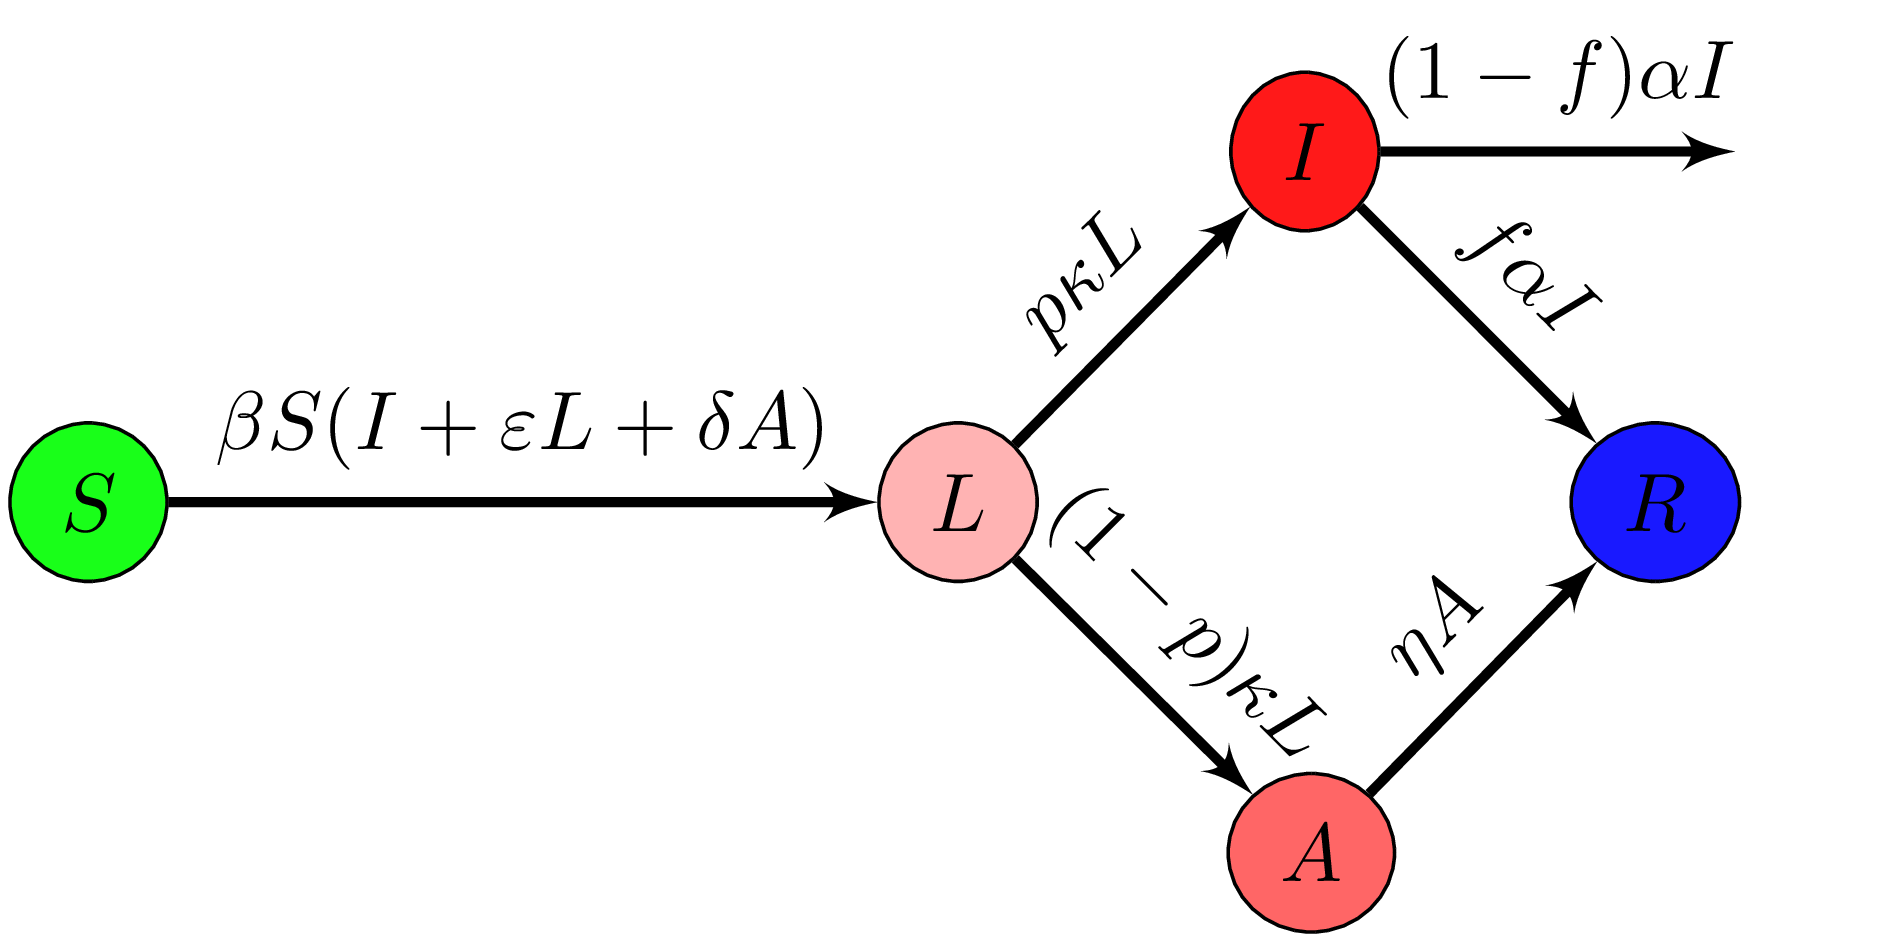
\includegraphics[width=\textwidth]{FIGS/SLIAR_infectiousL}
\end{frame}  


\begin{frame}
Here, $\bS=S$, $\bI=(L,I,A)^T$ and $\bR=R$, so $m=1$, $n=3$ and 
$$
\bh=[\varepsilon\; 1\; \delta],
\quad
\bD=1,
\quad 
\bPi
=\begin{pmatrix}
1 \\ 0 \\0
\end{pmatrix}
\quad\text{and}\quad
\mathbf{V}=
\begin{pmatrix}
\kappa & 0 & 0 \\
-p\kappa & \alpha & 0 \\
-(1-p)\kappa & 0 & \eta
\end{pmatrix}
$$
Incidence is mass action so $\beta(\bE_0)=\beta$ and thus
\begin{align*}
\mathcal{R}_0
&=
\beta\bh\mathbf{V}^{-1}\bPi\bD\bS_0 \\
&=
\beta\;
[\varepsilon\; 1\; \delta]
\begin{pmatrix}
1/\kappa & 0 & 0 \\
p/\alpha & 1/\alpha & 0 \\
(1-p)/\eta & 0 & 1/\eta
\end{pmatrix}
\begin{pmatrix}
1 \\ 0 \\0
\end{pmatrix}
S_0 \\
&=
\beta S_0\left(
\frac{\varepsilon}{\kappa}
+\frac{p}{\alpha}
+\frac{\delta(1-p)}{\eta}
\right)
\end{align*}
\end{frame}  

\begin{frame}
For final size, since $m=1$, we can use $\eqref{eq:final_size_m1}$:
\[
\ln\left(
\frac{S_0}{S_\infty}
\right)
=\frac{\mathcal{R}_0}{S_0}
(S_0-S_\infty)+\beta\bh\mathbf{V}^{-1}\bI_0
\]
\vfill
Suppose $\bI_0=(0,I_0,0)$, then
\[
\ln\left(
\frac{S_0}{S_\infty}
\right)
=\mathcal{R}_0\frac{S_0-S_\infty}{S_0}
+\frac{\beta}{\alpha}I_0
\]
\vfill
If $\bI_0=(L_0,I_0,A_0)$, then
\[
\ln\left(
\frac{S_0}{S_\infty}
\right)
=\mathcal{R}_0\frac{S_0-S_\infty}{S_0}
+\beta\left(
\frac{\varepsilon}{\kappa}
+\frac{p}{\alpha}
+\frac{\delta(1-p)}{\eta}
\right)L_0
+\frac{\beta\delta}{\eta}A_0
+\frac{\beta}{\alpha}I_0
\]
\end{frame}  



%%%%%%%%%%%%%%%%%%%%
%%%%%%%%%%%%%%%%%%%%
\subsection{A model with vaccination}
\newSubSectionSlide{FIGS-slides-admin/Gemini_Generated_Image_vqpscpvqpscpvqps.jpeg}

\begin{frame}{A model with vaccination}
\centering
\begin{tikzpicture}[auto, %node distance = 2cm, auto,
	cloud/.style={minimum width={width("N-1")+2pt},
		draw, ellipse,fill=gray!20}]
    \node [cloud, fill=green!90] (SU) {$S_U$};
    \node [cloud, below=2cmof SU, fill=green!90] (SV) {$S_V$};
    \node [cloud, right=3cm of SU, fill=red!30] (LU) {$L_U$};
    \node [cloud, right=3cm of SV, fill=red!30] (LV) {$L_V$};
	\node [cloud, right=of LU, fill=red!90] (IU) {$I_U$};
	\node [cloud, right=of LV, fill=red!90] (IV) {$I_V$};
	\node [cloud, below right=of IU, fill=blue!90] (R) {$R$};
    \node [cloud, above right=2cm of IU, draw=none, fill=none] (h1) {};
    \node [cloud, below right=2cm of IV, draw=none, fill=none] (h2) {};
	%% Infections
	\path [line, very thick] (SU) to node [midway, above] (TextNode) {$\beta S_U(I_U+\sigma_II_V)$} (LU);
	\path [line, very thick] (SV) to node [midway, above] (TextNode) {$\sigma_S\beta S_V(I_U+\sigma_II_V)$} (LV);
	\path [line, very thick] (LU) to node [midway, above, sloped] (TextNode) {$\kappa_U L_U$} (IU);
	\path [line, very thick] (LV) to node [midway, above, sloped] (TextNode) {$\kappa_V L_V$} (IV);
	\path [line, very thick] (IU) to node [midway, above, sloped] (TextNode) {$f_U\alpha_U I_U$} (R);
	\path [line, very thick] (IV) to node [midway, above, sloped] (TextNode) {$f_V\alpha_V I_V$} (R);
    \path [line, very thick] (IU) to node [midway, above, sloped] (TextNode) {$(1-f_U)\alpha_U I_U$} (h1);
    \path [line, very thick] (IV) to node [midway, below, sloped] (TextNode) {$(1-f_V)\alpha_V I_V$} (h2);
\end{tikzpicture}
\end{frame}  


\begin{frame}{A model with vaccination}
Fraction $\gamma$ of $S_0$ are vaccinated before the epidemic; vaccination reduces probability and duration of infection, infectiousness and reduces mortality
\begin{subequations}
\begin{align}
S_U\pprime &= -\beta S_U[I_U+\sigma_II_V] \\
S_V\pprime &= -\sigma_S\beta S_V[I_U+\sigma_II_V] \\
L_U\pprime &= \beta S_U[I_U+\sigma_II_V]-\kappa_UL_U\\
L_V\pprime &= \sigma_S\beta S_V[I_U+\sigma_II_V]-\kappa_VL_V \\
I_U\pprime &= \kappa_UL_U-\alpha_UI_U \\
I_V\pprime &= \kappa_VL_V-\alpha_VI_V \\
R\pprime &= f_U\alpha_UI_I+f_V\alpha_VI_V
\end{align}
\end{subequations}
with $S_U(0)=(1-\gamma)S_0$ and $S_V(0)=\gamma S_0$
\end{frame}  


\begin{frame}
Here, $m=2$, $n=4$,
\[
\bh = [0\;0\;1\;\sigma_I],\quad
\bD=\begin{pmatrix}
1 & 0 \\ 0 & \sigma_S
\end{pmatrix},\quad
\bPi=
\begin{pmatrix}
1 & 0 \\ 0 & 1 \\ 0 & 0 \\ 0 & 0
\end{pmatrix}
\]
and
\[
\mathbf{V}=
\begin{pmatrix}
\kappa_U & 0 & 0 & 0 \\
0 & \kappa_V & 0 & 0 \\
-\kappa_U & 0 & \alpha_U & 0 \\
0 & -\kappa_V & 0 & \alpha_V
\end{pmatrix}
\]
\end{frame}

\begin{frame}
So
\[
\bGamma=\left[
\frac{\beta}{\alpha_U}\; \frac{\sigma_I\sigma_S\beta}{\alpha_V}
\right],
\quad
\mathcal{R}_c = S_0\beta\left(
\frac{1-\gamma}{\alpha_U}+\frac{\sigma_I\sigma_S\gamma}{\alpha_V}
\right)
\]
and the final size relation is
\begin{multline*}
\ln\left(
\frac{(1-\gamma)S_U(0)}{S_U(\infty)}
\right)
= \\ 
\frac{\beta}{\alpha_U}[(1-\gamma)S_U(0)-S_U(\infty)] \\
+\frac{\sigma_I\beta}{\alpha_V}[\gamma S_V(0)-S_V(\infty)]+\frac{\beta}{\alpha_U}I_0 \\
\end{multline*}
\[
S_V(\infty) = \gamma S_U(0)\left(
\frac{S_U(\infty)}{(1-\gamma)S_0}
\right)^{\sigma_S}
\]
\end{frame}

%%%%%%%%%%%%%%%%%%%%
%%%%%%%%%%%%%%%%%%%%
\subsection{Antiviral resistance}
\newSubSectionSlide{FIGS-slides-admin/Gemini_Generated_Image_vqpscpvqpscpvqps.jpeg}

\maxFrameImage{FIGS/ArinoBowmanMoghadas.png}
\nocite{ArinoBowmanMoghadas2009}

\begin{frame}{Adapting treatment to counter emergence of resistance}
This work was undertaken at the request of the Public Health Agency of Canada during the pandemic preparadness phase prior to the 2009 p-H1N1 pandemic
\vfill
Problem: we have antivirals to use against influenza, either prophylactically or curatively. Using these antivirals may promote the emergence of antiviral-resistant strains. How do we minimise this risk?
\end{frame}


\begin{frame}
\centering
\resizebox{\textwidth}{!}{
  \begin{tikzpicture}[%transform canvas={scale=1.3},
      auto,
      cloud/.style={minimum width={width("N-1")+2pt},
      draw, 
      ellipse,
      fill=gray!20}]
    %% S
    \node [cloud, fill=green!90] at (0,0) (S) {$S$};
    %% Untreated, resistant
    \node [cloud, fill=red!90] at (3,1) (A_r) {$A_r$};
    \node [cloud, fill=red!60] at (3,-1) (I_rU) {$I_{rU}$};
    \node [cloud, fill=blue!60] at (6,0) (R_rU) {$R_{rU}$};
    %% Untreated, sensitive
    \node [cloud, fill=red!90] at (-3,1) (A) {$A$};
    \node [cloud, fill=red!60] at (-3,-1) (I_U) {$I_U$};
    \node [cloud, fill=blue!60] at (-6,0) (R_U) {$R_U$};
    %% Treated
    \node [cloud, fill=red!90] at (-1.5,-3) (I_T) {$I_T$};
    \node [cloud, fill=red!90] at (1.5,-3) (I_rT) {$I_{rT}$};
    \node [cloud, fill=red!90] at (0,-6) (I_Tr) {$I_{Tr}$};
    %% Resistance
    \node [cloud, fill=blue!60] at (-4.5,-3) (R_T) {$R_T$};
    \node [cloud, fill=blue!60] at (4.5,-3) (R_rT) {$R_{rT}$};
    \node [cloud, fill=blue!60] at (3,-6) (R_Tr) {$R_{Tr}$};
    %%
    %% Infections
    \path [line, very thick] (S) to node [midway,above,sloped] (TextNode) {$(1-p)fS$} (A);
    \path [line, very thick] (S) to node [midway,below,sloped] (TextNode) {$(1-q)pfS$} (I_U);
    \path [line, very thick] (S) to node [midway,above,sloped] (TextNode) {$(1-p)gS$} (A_r);
    \path [line, very thick] (S) to node [midway,below,sloped] (TextNode) {$(1-q)pgS$} (I_rU);
    \path [line, very thick] (S) to node [near end,above,sloped] (TextNode) {$qpfS$} (I_T);
    \path [line, very thick] (S) to node [midway,below,sloped] (TextNode) {$qpgS$} (I_rT);
    %% Removals
    \path [line, very thick] (A) to node [midway,below,sloped] (TextNode) {$\mu_AA$} (R_U);
    \path [line, very thick] (I_U) to node [midway,below,sloped] (TextNode) {$(d_U+\mu_U)I_U$} (R_U);
    \path [line, very thick] (A_r) to node [midway,below,sloped] (TextNode) {$\mu_AA_r$} (R_rU);
    \path [line, very thick] (I_rU) to node [midway,below,sloped] (TextNode) {$(d_{rU}+\mu_U)I_{rU}$} (R_rU);
    \path [line, very thick] (I_T) to node [midway,below,sloped] (TextNode) {$(d_T+\mu_T)I_T$} (R_T);
    \path [line, very thick] (I_rT) to node [midway,below,sloped] (TextNode) {$(d_{rU}+\mu_U)I_{rT}$} (R_rT);
    \path [line, very thick] (I_Tr) to node [midway,below,sloped] (TextNode) {$(d_{Ur}+\mu_U)I_{Tr}$} (R_Tr);
    %% I_T transitions
        \path [line, very thick] (I_T) to node [midway,below,sloped] (TextNode) {$\alpha I_T$} (I_Tr);
    \path [line, very thick] (I_Tr) to node [midway,below,sloped] (TextNode) {$\gamma I_{Tr}$} (I_rT);
  \end{tikzpicture}
}
\end{frame}




%%%%%%%%%%%%%%%%%%%%%%%%%%
%%%%%%%%%%%%%%%%%%%%%%%%%%
%%%%%%%%%%%%%%%%%%%%%%%%%%
%%%%%%%%%%%%%%%%%%%%%%%%%%


%%%%%%%%%%%%%%%%%%%%%%%%%%
%%%%%%%%%%%%%%%%%%%%%%%%%%
%%%%%%%%%%%%%%%%%%%%%%%%%%
%%%%%%%%%%%%%%%%%%%%%%%%%%
\begin{frame}[allowframebreaks]{Bibliography}
\bibliographystyle{plain}
\bibliography{local-bibliography}
\end{frame}

\end{document}
